\documentclass[a4paper,11pt]{article}

\usepackage[utf8]{inputenc}
\usepackage[T1]{fontenc}
\usepackage[francais]{babel}
\usepackage{fancyhdr}
\usepackage{graphicx}
\usepackage{float}
\usepackage{lastpage}
\usepackage{amssymb}
\usepackage{amsmath}
\usepackage{url}
\usepackage{textcomp}
\usepackage{gensymb}
\usepackage{array}
 %\usepackage{mathrsfs}
\usepackage{epstopdf}
%\usepackage{hyperref}%ugly link
\usepackage[top=3cm, bottom=3cm, left=2cm, right=2cm]{geometry}
\pagestyle{fancy}
\headheight=15pt
\parskip=6pt
\parindent=10pt

\title{ \vspace{2ex}
Utiliser une
\\ \vspace{5ex} \Huge{\textbf{
Imprimante 3D
}}}
\author{Gaétan Collaud}
\date{\vspace{1ex}\today}
\lhead{Fablab Fribourg} \chead{} \rhead{Imprimante 3D}
\lfoot{Gaétan Collaud} \cfoot{} \rfoot{\thepage/\pageref{LastPage}}


\begin{document}

\maketitle

\vspace{10ex}

\begin{figure}[H]
	\centering
	\includegraphics[scale=1]{fablab_fribourg_rouge.eps}
\end{figure}

\thispagestyle{empty}	

\newpage
\tableofcontents
\newpage

\section{Introduction}

Ce document décrit comment utiliser une imprimante au Fablab Fribourg. Les photos seront tirées de l’imprimante Ultimaker V1. Mais les principes restent les mêmes pour n’importe quelle imprimante.

 % !TEX root = ../imprimante3d.tex

\section{Sécurité}

\subsection{Électrocution}

L’alimentation de l’imprimante ainsi que du lit chauffant est en dessous de 50V. Il n’y a donc, normalement, aucun risque d’électrocution.

\subsection{Brulure}

\subsubsection{Tête d'impression}

La tête d’impression est très chaude lors du fonctionnement, de l’ordre de 220 à 270°C . Il faut donc faire attention à ne pas mettre les doigts contre (c'est vite arrivé surtout quand on bidouille).

\subsubsection{Lit chauffant}

Le lit chauffant n'est pas forcément présent sur toutes les machines. Le lit chauffant peut attendre jusqu'à 100°C (même si en général il ne dépasse pas 70°C). Là encore il y a le risque de se brûler. C'est moins grave qu'avec la tête, mais il faut faire attention. Le lit chauffant est comparable à une plaque de cuisson, si on s'en approche, on sent très bien la chaleur.


 % !TEX root = ../imprimante3d.tex

\section{Matériel}

Ce chapitre décrit les différentes parties de l'imprimante et leur utilité. Encore une fois les illustrations montrent une Ultimaker mais les autres imprimantes ne sont pas si différentes.

\subsection{Contrôleur}

Le contrôleur est l'interface de l'imprimante. S'il n'y en a pas, cela signifie que l'imprimante se pilote directement depuis l'ordinateur. Un contrôleur permet à l'imprimante d'être totalement autonome. On peut également la configurer avant et pendant une impression. Lors d'une impression ce contrôleur nous indique la température des différents éléments, l'état d'avancement de l'impression et le temps écoulé.

\begin{figure}[H]
	\centering
	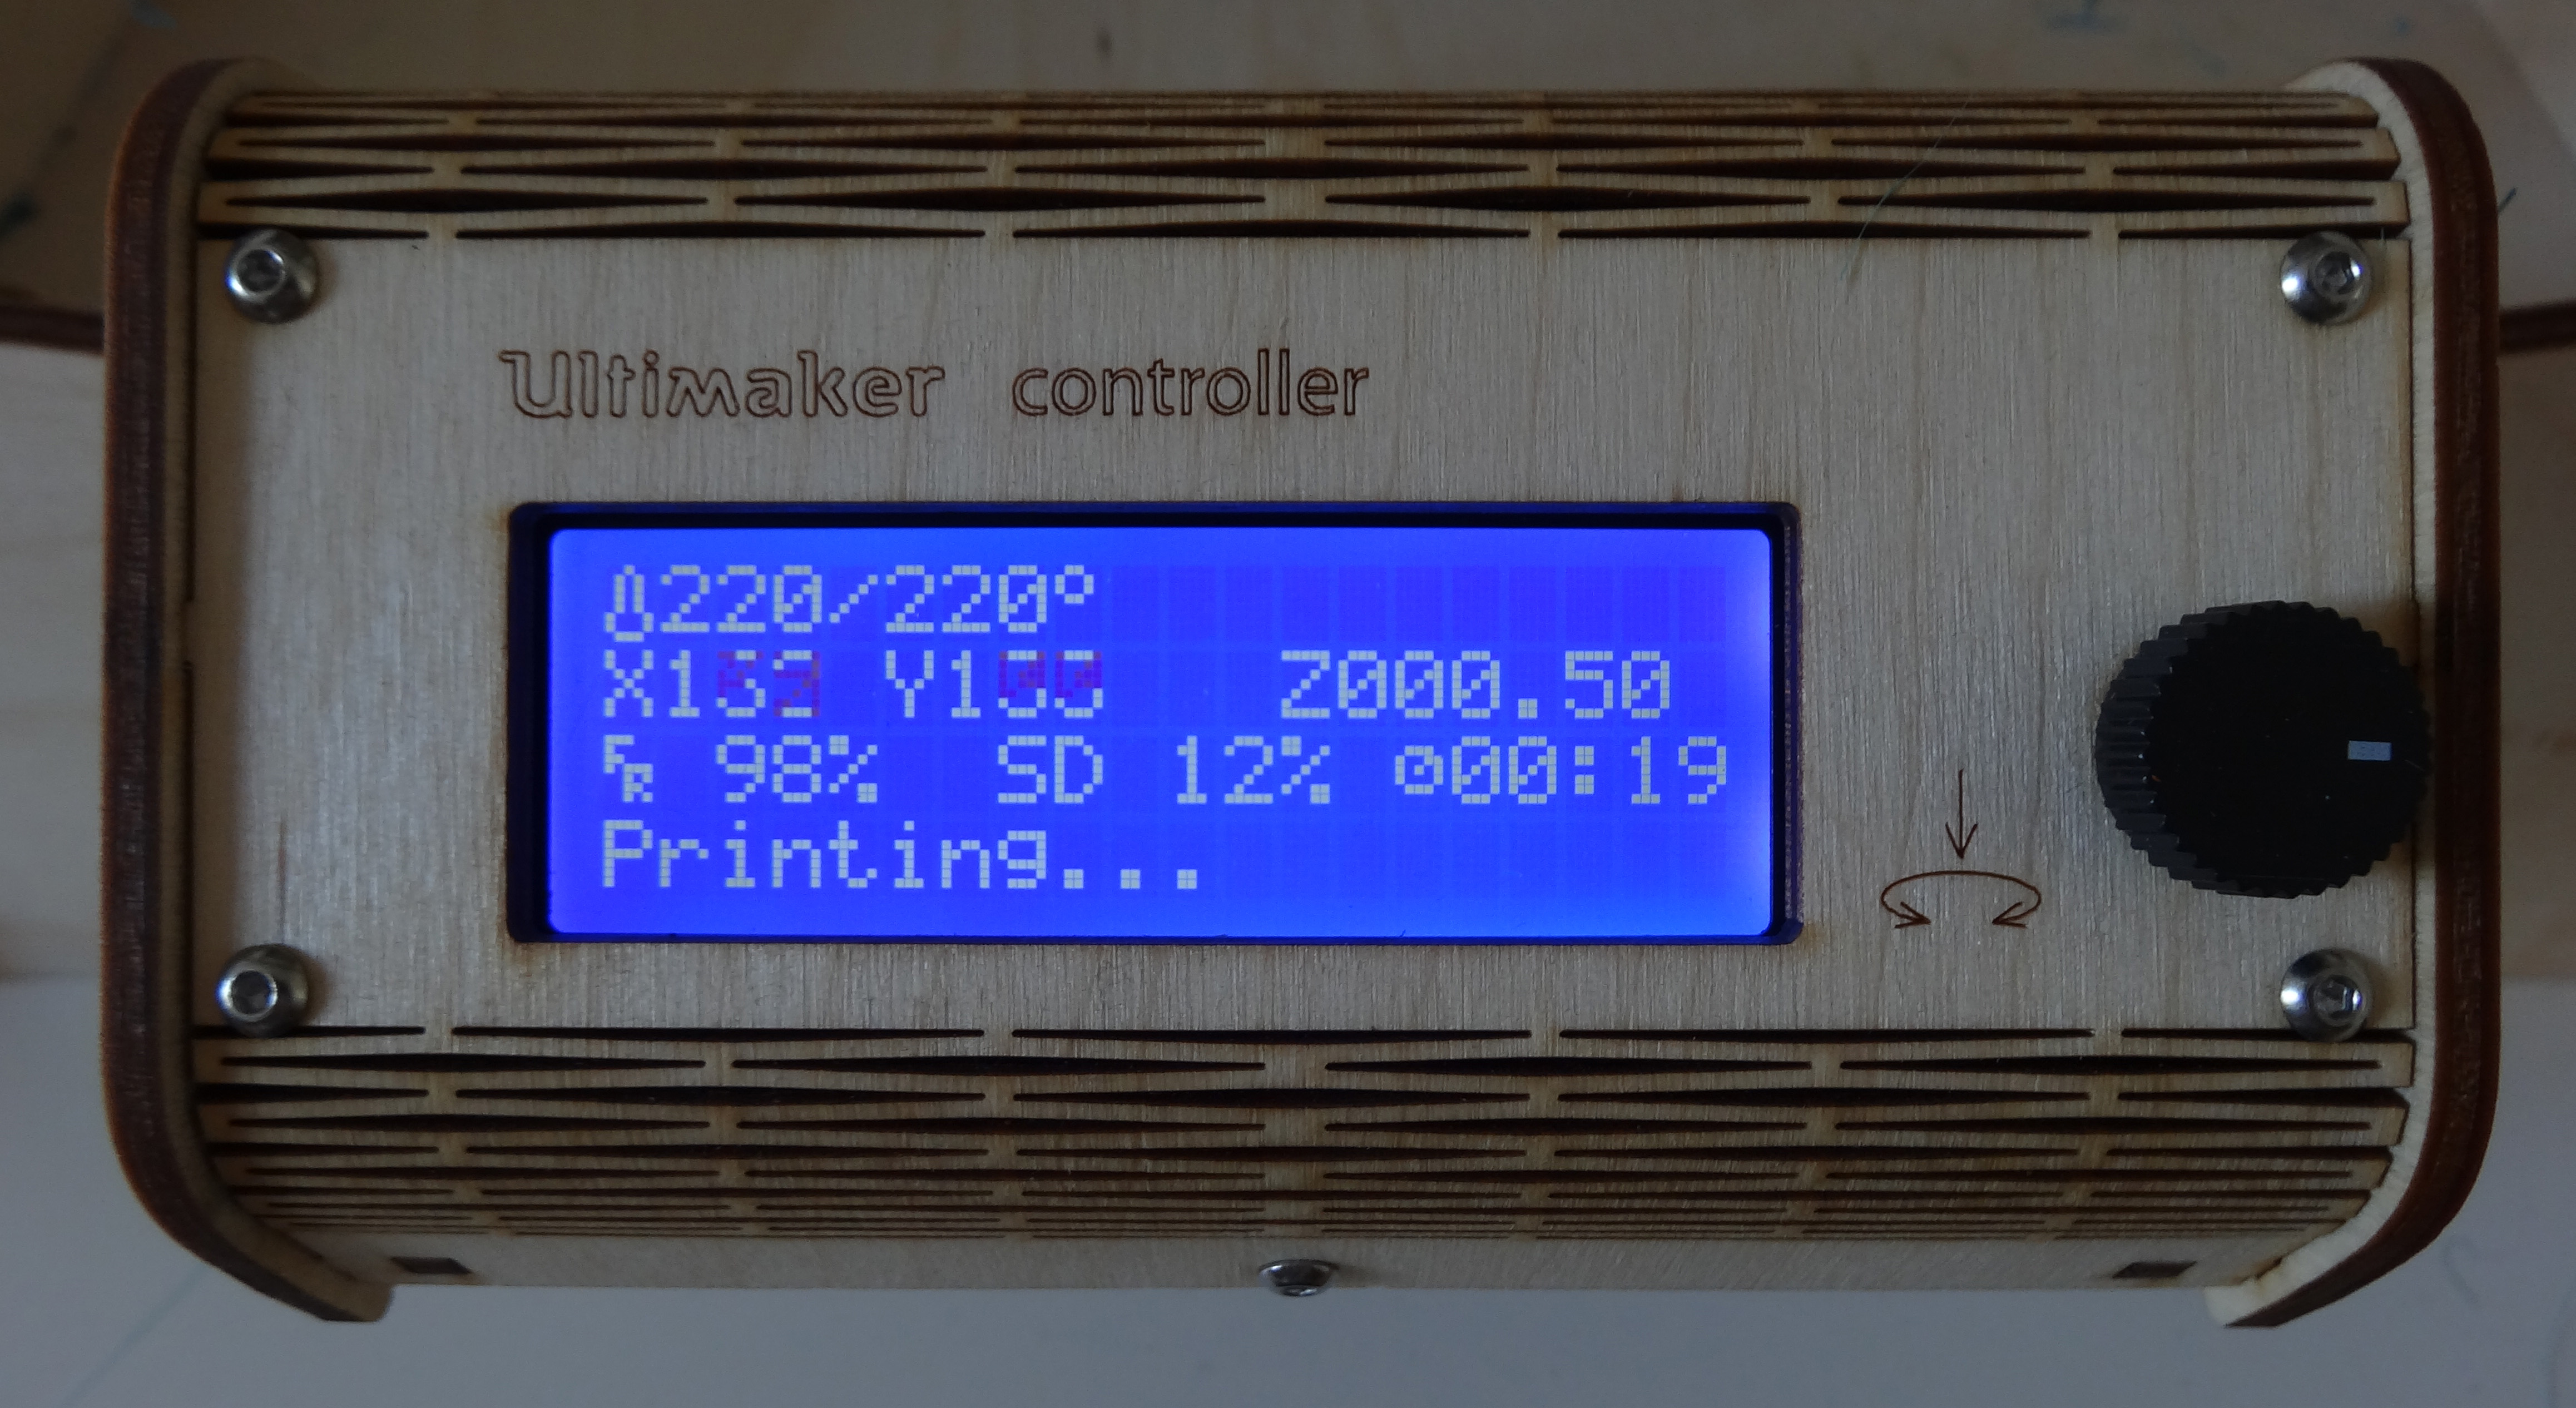
\includegraphics[width=50ex]{02_materiel/controller.jpg}  
	\caption{Contrôleur de l'Ultimaker V1}
	\label{fig:controller}
\end{figure}

\paragraph{} Concernant l'état d'avancement, il s'agit de l'avancement dans le fichier contenant le GCode (le code machine). Il ne faut pas prendre cette information trop sérieusement. Elle ne correspond pas au pourcentage de temps écoulé. C'est juste une indication. Pour connaitre ne approximation du temps d'impression, il faut regarder le temps indiqué dans les logiciels (même si celui-ci n'est pas forcément très précis).

\subsection{Tête d'impression}

La tête d'impression sert à faire fondre le filament et le déposer couche par couche. Elle fait usuellement $400\mu$ de diamètre. Le plateau doit être calibré de sorte à frôler la tête d'impression en tout points du plateau. Pour vérifier ceci, il suffit de faire un \emph{Auto Home} avec le contrôleur ou l'ordinateur de sorte à remettre l'imprimante à sa position de départ. Ensuite on déplace gentiment à la main la tête sur le plateau pour voir si le plateau est bien calibré. Si ce n'est pas le cas, il faut s'aider des vis dans les coins pour l'ajuster.

\begin{figure}[H]
	\centering
	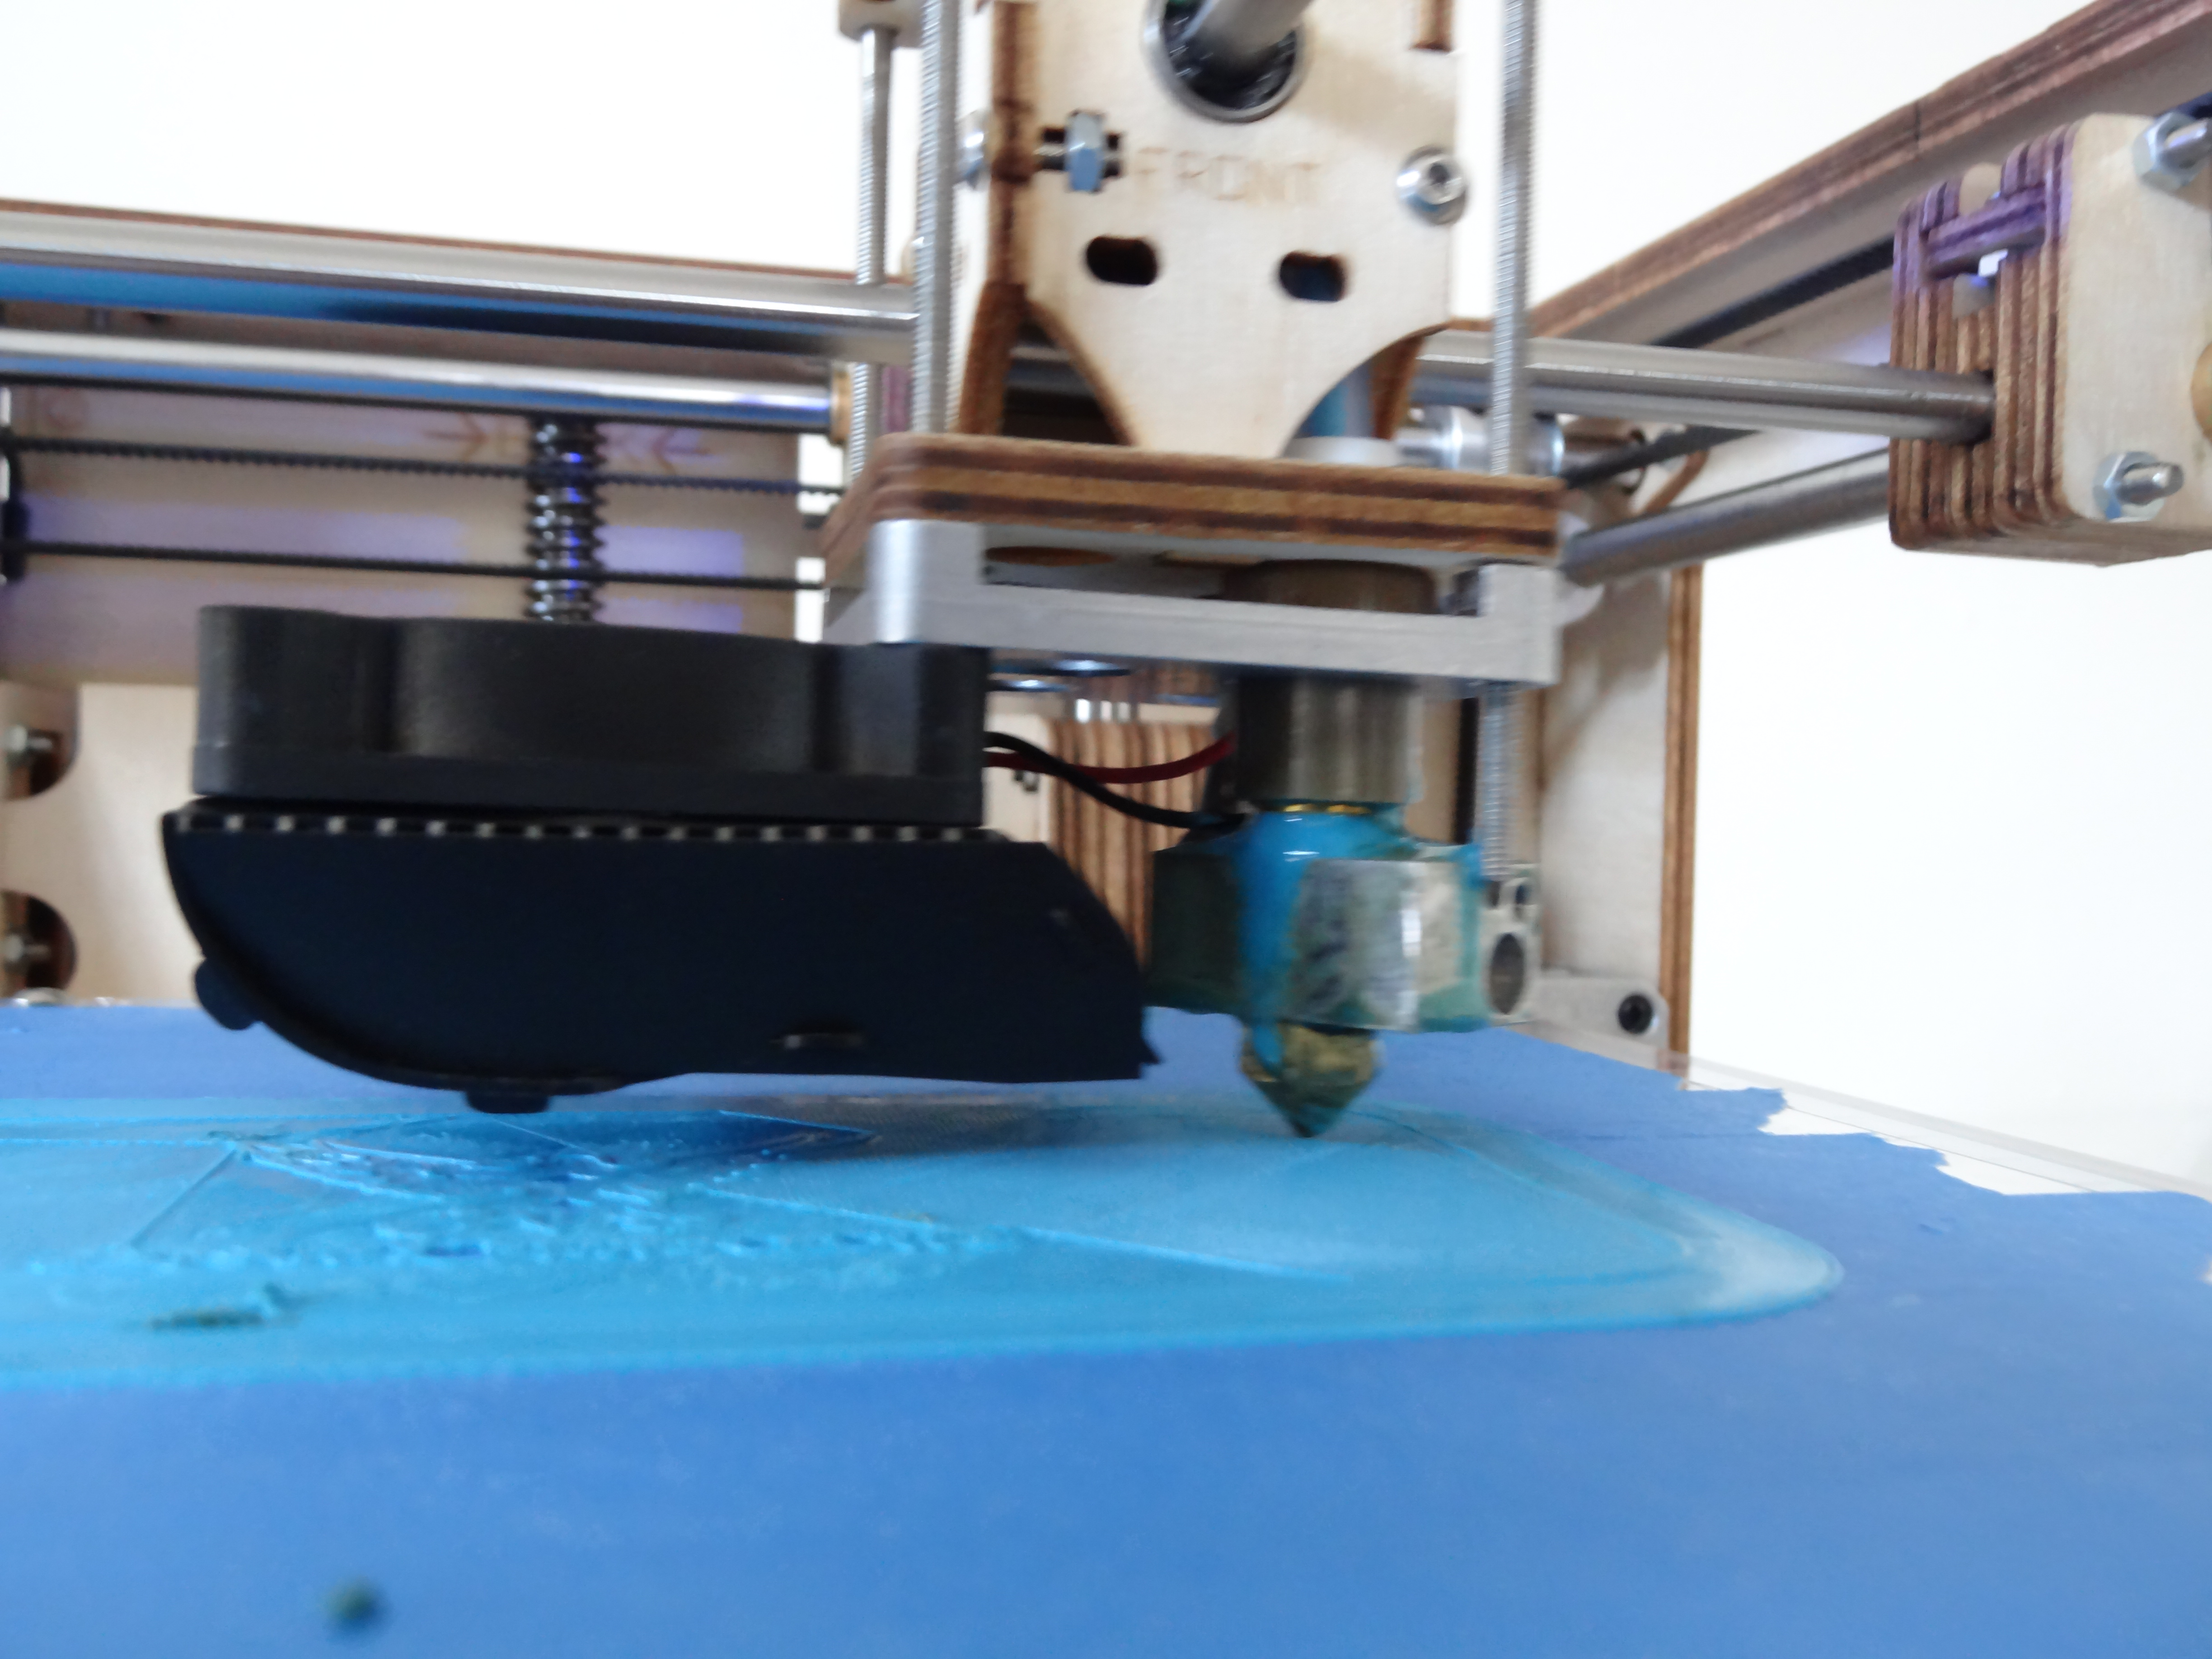
\includegraphics[width=50ex]{02_materiel/head1.jpg}  
	\caption{Tête d'impression de l'Ultimaker V1}
	\label{fig:head1}
\end{figure}

\subsection{Plateau}

\subsection{Scotch d'adhésion}

S'il n'y a pas de lit chauffant, le plateau est normalement recouvert d'un scotch aidant à l'adhésion de la pièce sur le plateau. Ce scotch se dégrade au fil du temps et doit être remplacé. Pour se faire, il suffit simplement d'enlever le plateau de l'imprimante et de remplacer le scotch à la main. Il y a des guides sur le plateau pour faciliter la découpe au cutter. Après cette opération, il ne faut pas oublier de recalibrer le plateau si cela s'avère nécessaire. A la fin d'une impression, la pièce peut être difficile à enlever. On peut s'aider d'un couteau pour faire décoller un coin de la pièce et le reste devrait venir assez facilement ensuite.

\subsection{Lit chauffant}

Le but du lit chauffant est de faire adhérer la matière au plateau tout au long de l'impression. Il ne faut surtout pas le désactiver en cours de route. La température du lit dépend de la matière que l'on imprime. Pour du PLA, il faut le mettre entre 60 et 70°C, mais pour de l'ABS, cela se situe plus autour des 100°C. A la fin de l'impression, il faut attendre que le lit refroidissent. Une fois que le lit est froid la pièce se décollera d'elle-même.

\subsection{Moteurs}

Les moteurs présents sur les imprimantes sont souvent des moteurs dits pas-à-pas. C'est-à-dire qu'ils ont des \emph{crans} tout les tant de degrés. Ils ont l'avantage d'être peu cher pour leur précision. 

 \paragraph{} Par contre il peut arriver qu'un moteur \emph{saute} ou loupe un ou plusieurs pas. Ceci est très mauvais, car l'imprimante ne saura pas qu'elle a glissé. L'imprimante envoie des commandes au moteur en lui disant le nombre de pas à avancer ou reculer. Si le moteur saute un pas, l'imprimante sera perdue et l'impression ne ressemblera à rien. On retrouve ce problème sur les CNC par exemple. Quand un moteur saute un pas, il faut un bruit spécial très distinct. Si cela arrive, il faut arrêter l'impression. Éventuellement graisser les axes et recommencer. L'environnement d'un Fablab est très poussiéreux, il peut donc arriver qu'un roulement devienne sale et qu'il faille le graisser (voir même le changer).

\subsubsection{Extrudeur}

Le moteur d'extrusion se trouve à l'arrière de l'Ultimaker. Pour les autres imprimantes, il se situe souvent sur la tête d'impression. Ce moteur pousse la matière dans la tête d'impression. Si le moteur n'est pas allumé, on peut sans autre tournée la rue pour pousser manuellement le filament. Comme on peut le voir sur la figure \ref{fig:extruder}, il y a une petite flèche pour indiquer le sens dans lequel tourner pour extraire de la matière.

\begin{figure}[H]
	\centering
	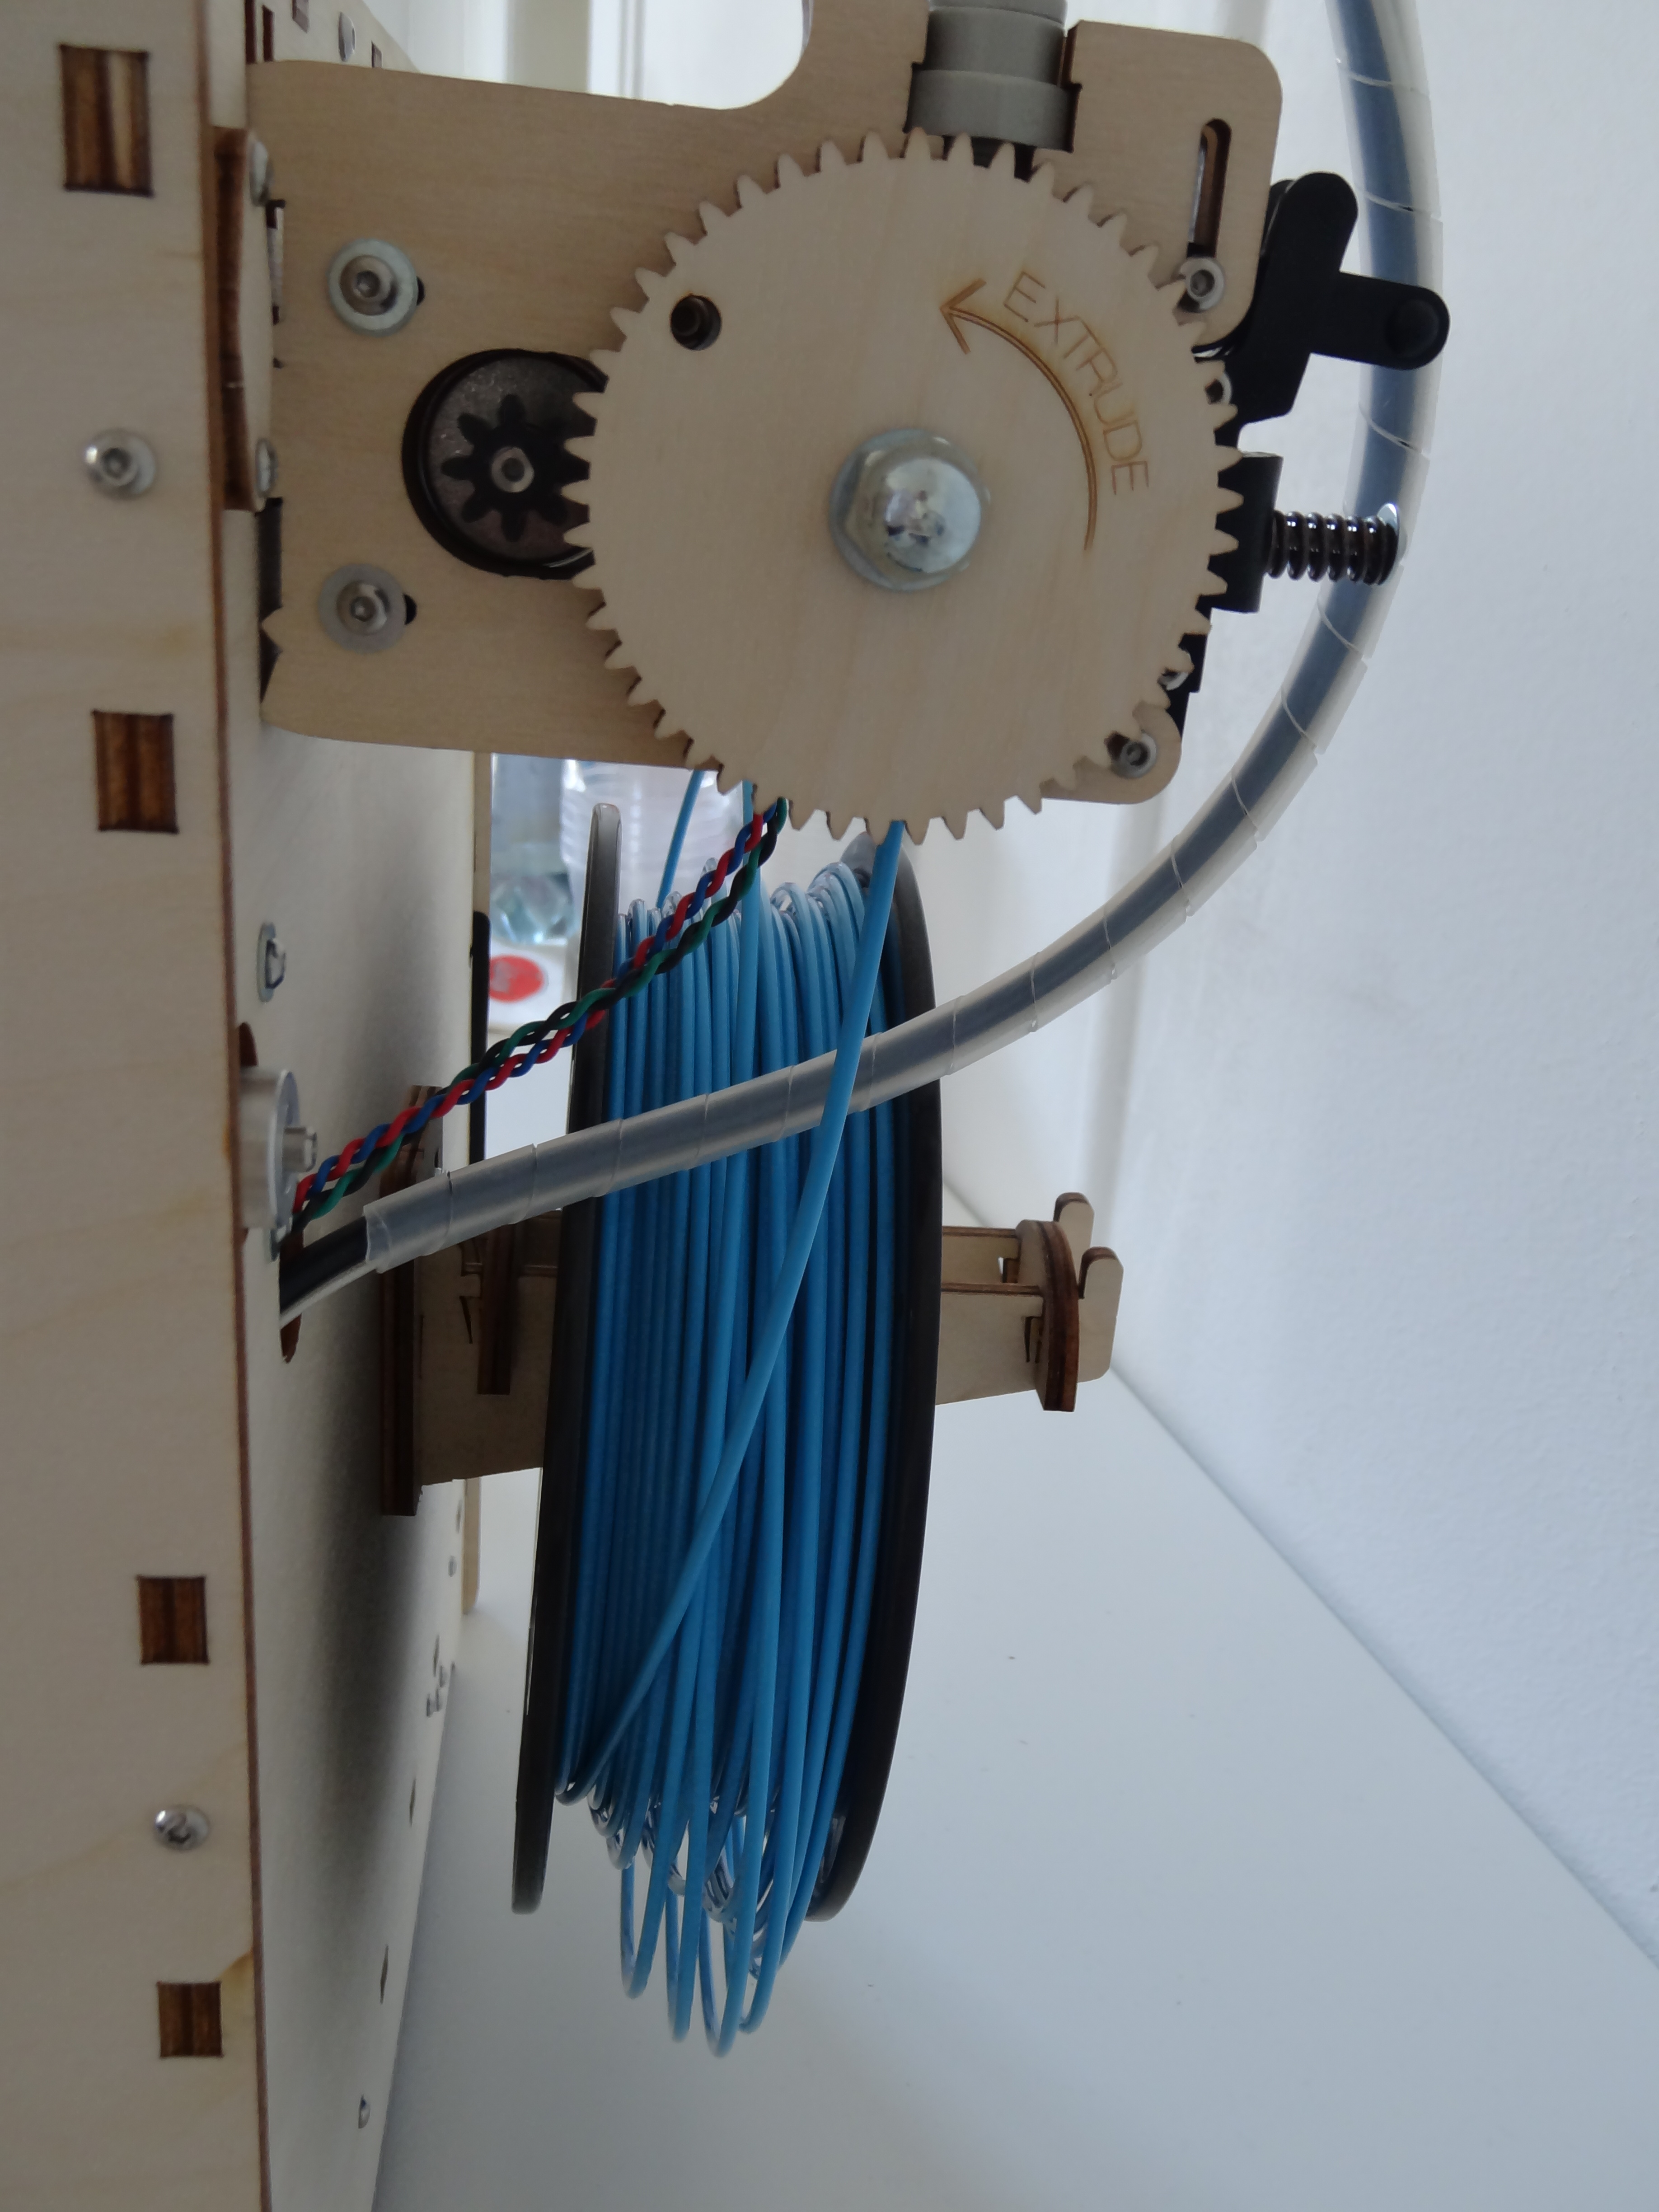
\includegraphics[width=50ex]{02_materiel/extruder.jpg}  
	\caption{Extrudeur et bobine sur l'Ultimaker V1}
	\label{fig:extruder}
\end{figure}

\subsubsection{Moteur x y z}

Ces moteurs servent à faire bouger la tête d'impression et le plateau. Sur l'Ultimaker, le plateau bouge en Z (en hauteur) et la tête en X (largeur) et Y (profondeur). Mais toutes les configurations sont possibles. Comme dit plus haut, il est possible que ces moteurs sautent des pas. Dans ce cas il faut graisser les roulements. Ne jamais graisser le moteur lui-même !



 % !TEX root = ../imprimante3d.tex

\section{Logiciel}

Ce chapitre reprend les grandes lignes des logiciels permettant de convertir un objet 3D en Gcode pour l'imprimante. Nous verrons ensuite plus en détail le logiciel Cura d'Ultimaker. L'objet 3D à imprimer doit être au préalable dans un format standard tel que STL ou OBJ. N'importe quel logiciel de modélisation 3D devrait être capable d'enregistrer ou d'exporter un objet dans l'un de ces deux formats.

\subsection{Concepts}

Voici quelques concepts qu'il faudrait connaitre pour bien paramétrer sont imprimante. Si vous n'utiliser pas les logiciels en mode expert et que vous n'utilisez que les options de base, passez votre chemin.

\subsubsection{Qualité}

La qualité d'une impression dépend surtout de l'imprimante en elle-même. Cependant on peut jouer avec la hauteur des couches pour avoir une meilleure qualité. Pour un brouillon, on peut mettre $2.5mm$, pour une qualité normal, on mettra plutôt $2mm$. Pour une bonne qualité, on utilise $1mm$. On peut aller plus bas encore, mais cela ne change plus grand chose. Il faut savoir que plus les couches sont fines, plus il faudra en faire et donc plus l'impression sera longue.

\paragraph{} Si l'objet ne parait pas assez remplis sur les couches inférieures ou supérieur, le flux est peut-être mal régler. On peut changer le flux directement pendant une impression avec le contrôleur (pour l'Ultimaker du moins). Sinon on peut jouer avec les paramètres de diamètre et densité du filament pour avoir plus ou moins de matières déposées à chaque passage.

\subsubsection{Vitesse}

Une vitesse standard pour une impression est autour de $50mm/s$. La encore une fois tout dépend de l'imprimante. L'Ultimaker peut aller facilement jusqu'à $150mm/s$ du fait se sont faible poids de sa tête (dû à l'extrudeur placé en dehors). Une grande vitesse pourra avoir une influence négative sur la qualité de l'objet. Pour l'ultimaker une vitesse de $80mm/s$ est une bonne valeur.

\paragraph{} Dans les paramètres avancés, on peut également régler la vitesse de la première couche. Cette couche est très importante vue qu'elle sera responsable de l'adhésion de la pièce. Une vitesse inférieure à la vitesse normale d'impression est donc appliquée. Une vitesse de $20mm/s$ est une valeur standard pour la première couche.

\subsubsection{Adhésion}

Dans certains logiciels comme curra, il est possible d'utiliser une technique d'adhésion particulière. Ces techniques servent à ce que la pièce tienne bien en place sur le plateau. Il est très important d'en ajouter une quand la pièce est grande, mais que la surface d'adhésion est petite.

\begin{description}
\item [Brim] ajoute plusieurs lignes tout autour de la pièce. On peut facilement enlever cette couche supplémentaire sans pour autant détériorer la pièce. 
\item[Raft] ajoute un \emph{radeau} sous la pièce. Fonctionne bien, mais il faudra raboter le fond de la pièce après l'impression. L'état de surface ne sera pas forcément très lisse.
\end{description}

Dans la plupart des cas, on utilise \emph{brim}.

\begin{figure}[H]
	\centering
	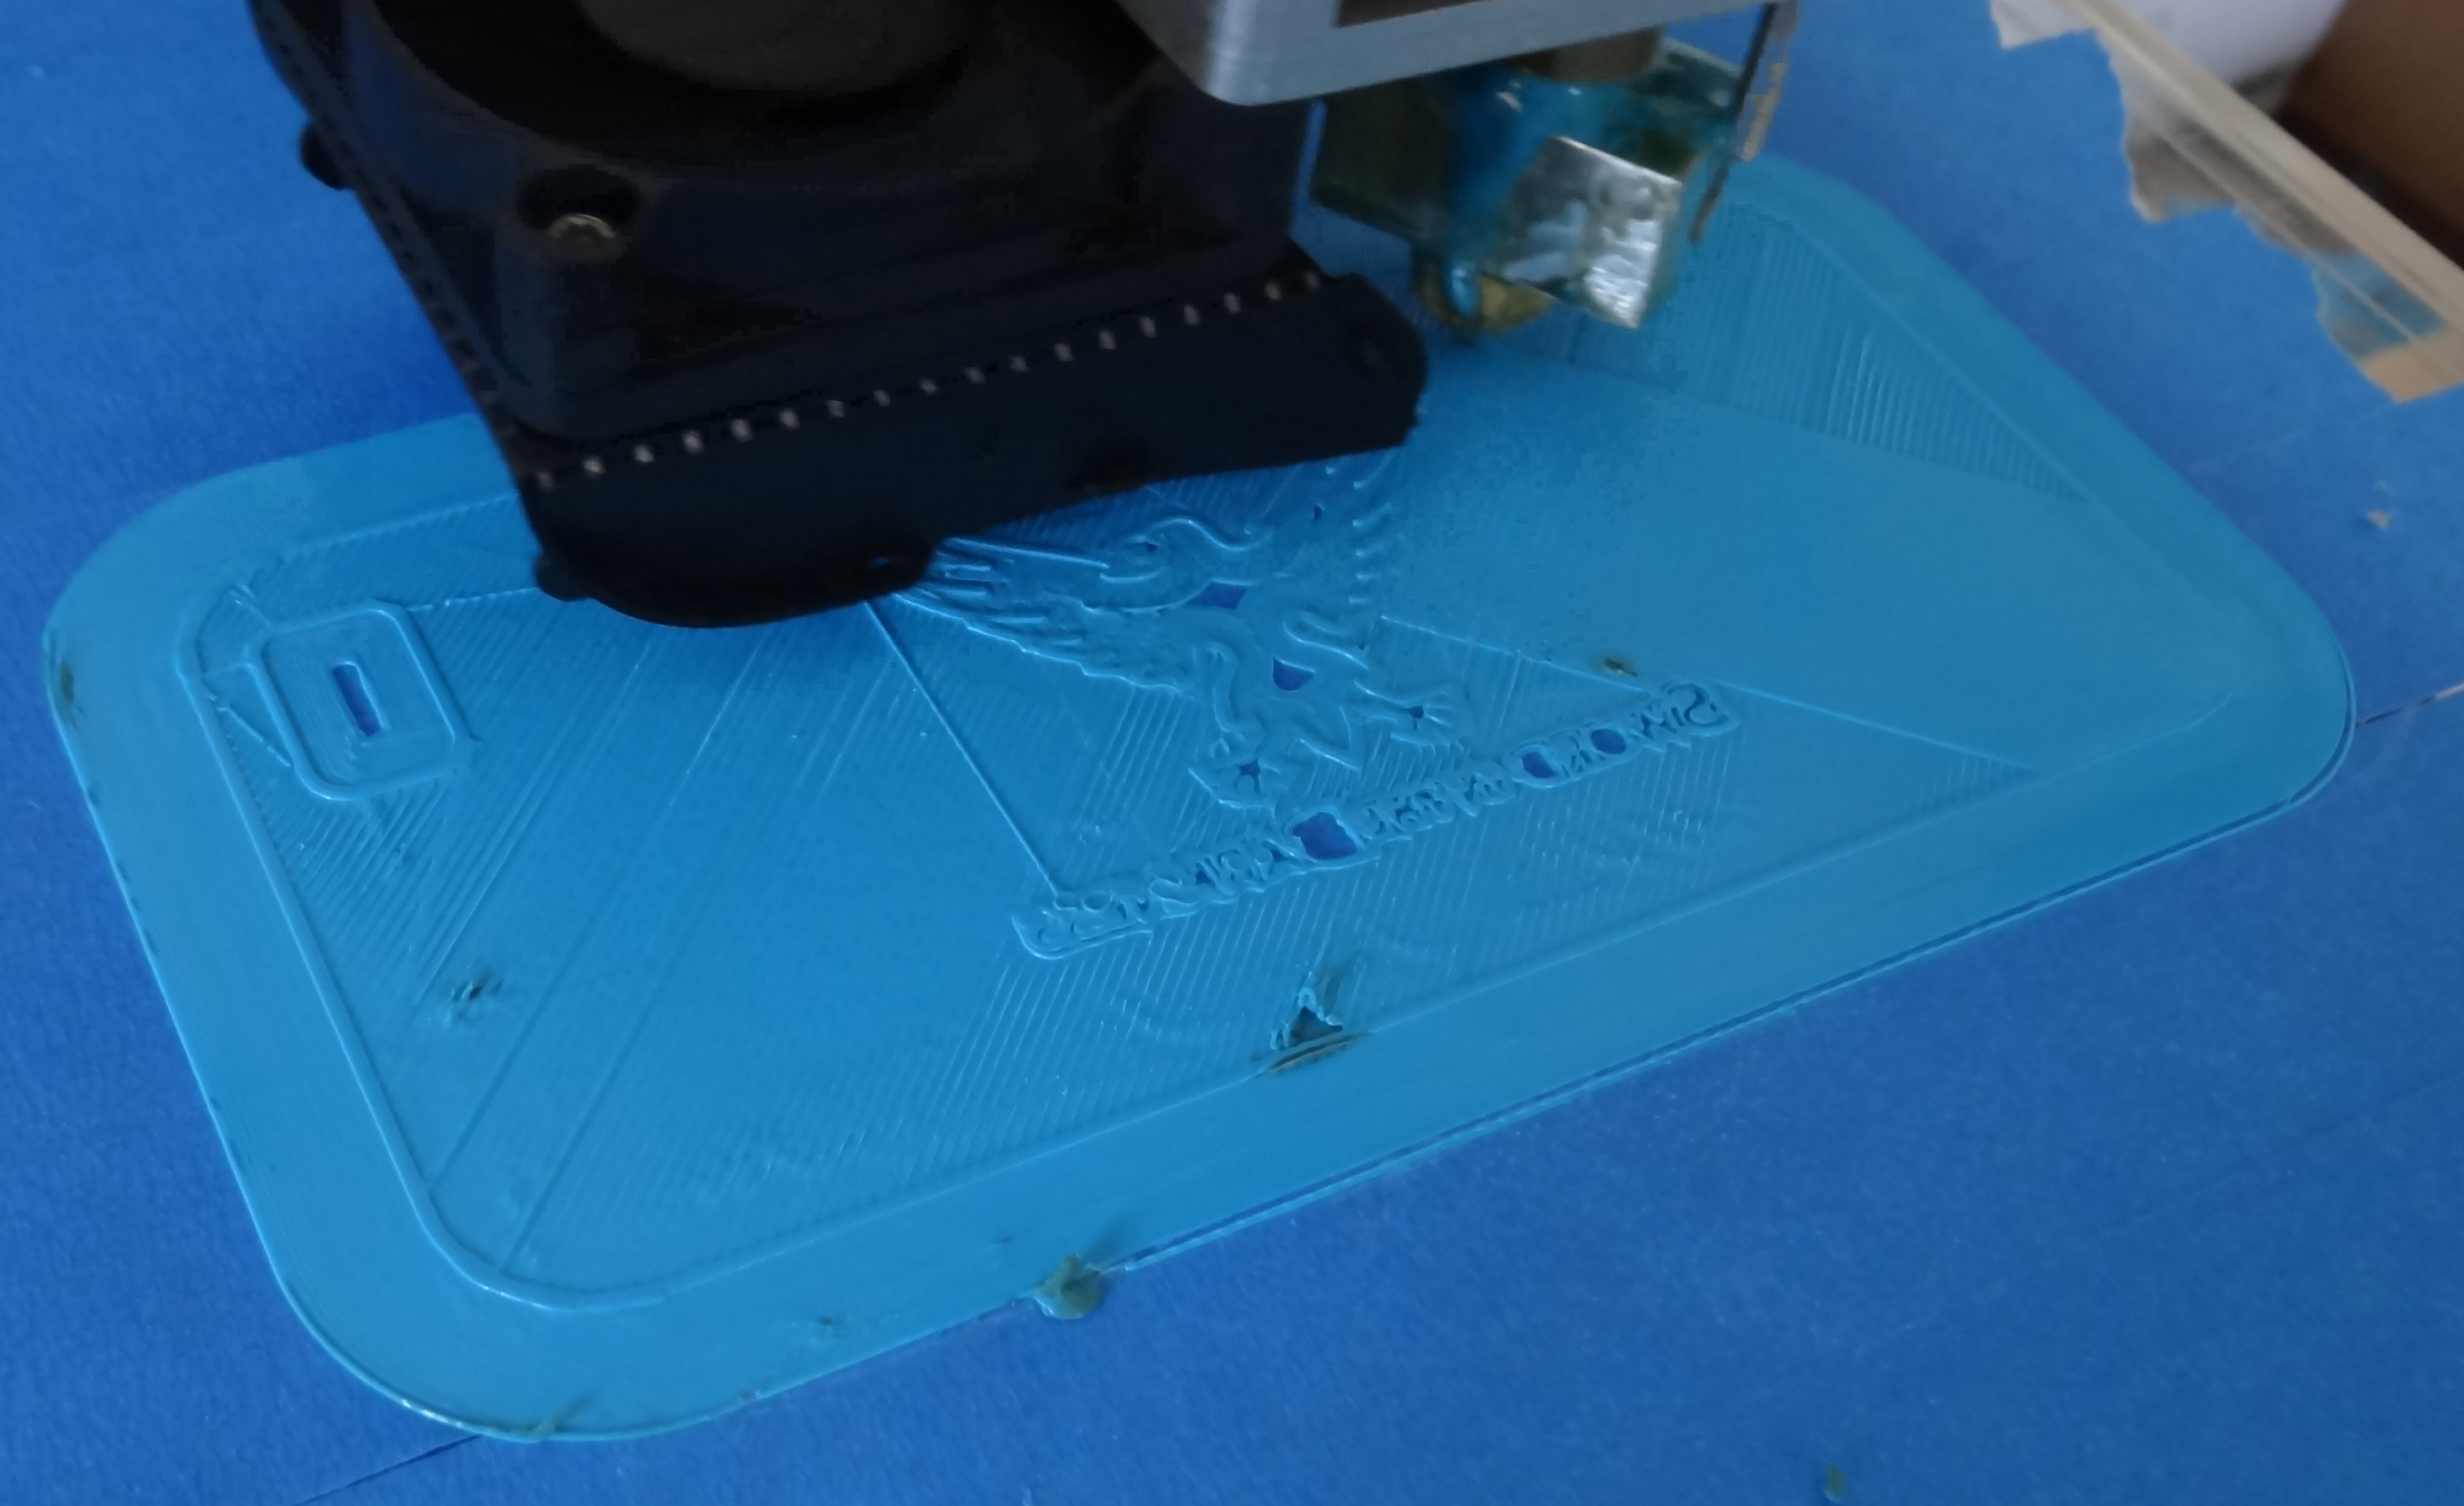
\includegraphics[width=50ex]{03_logiciel/brim.jpg}  
	\caption{Adhésion : brim}
	\label{fig:brim}
\end{figure}

Sur la figure \ref{fig:brim} on peut clairement voir qu'une couche à été rajouter tout autour de l'objet (ici, une coque d'Iphone).

\subsubsection{Support}

Une imprimante 3D imprime de bas en haut. S'il arrive que pour un objet on doive démarré l'impression d'une de ses parties dans le vide, il faut ajouter un support. Ce support pourra être facilement enlevé après l'impression. Il y a plusieurs types de support :

\begin{description}
\item [Touching buildplate] Ajoute un support uniquement entre le plateau et la pièce (si besoin)
\item[Everywhere] Ajoute en plus un support à l'intérieur de la pièce (si cela est nécessaire)
\end{description}

Il n'y a pas de valeur par défaut ici, il faut voir au cas par cas. Mais pour le $90\%$ des pièces, aucun support n'est requis.

\subsection{Cura}

\subsubsection{Mode}

\begin{description}
\item [Quickprint] (Impression rapide) Ce mode ne permet que de choisir entre bonne, normale et basse qualité. Cura adaptera tous les paramètres pour vous. On peut voir ça comme un mode automatique
\item[Full settings] (Toutes les options) Ce mode donnes accès à tous les paramètres avancés de l'application.
\end{description}

\subsubsection{Paramètres}
Sur la gauche de Cura se trouvent les paramètres d'impression. Ils ne seront pas tous détaillés ici. On retrouve notamment les paramètres des concepts expliqués précédemment.

\subsubsection{Différentes vues 3D}
La vue 3D nous donne une vue de l'imprimante et de la pièce que l'on va imprimer. La couleur n'a bien entendu rien à voir, elle dépend uniquement du filament installé.

\paragraph{} En haut à droite, on a un bouton pour choisir le type de vue que l'on veut. Une vue qui peut s'avérer utile est la vue \emph{Layers} (couches). Elle montre couche par couche la trajectoire que Cura a calculée.


\subsubsection{Éditer la pièce}

Nous pouvons éditer basiquement la pièce directement depuis Cura. C'est-à-dire que nous pouvons l'agrandir ou rétrécir (\emph{Scale}), nous pouvons la retourner (\emph{Rotation}) et nous pouvons lui appliquer des effets de miroir (\emph{Mirror}). Toutes ces actions peuvent être effectuées à l'aide des boutons en bas à gauche de la Vue 3D.

\subsubsection{Exporter pour imprimer}

A l'aide des boutons en haut à gauche, nous pouvons enregistrer le GCode (le code machine). Le Gcode peut-être placé sur une carte SD pour ensuite être introduite dans le contrôleur. Si l'imprimante est directement connectée, on peut également lancer l'impression directement depuis Cura.

\subsubsection{Estimations}

Cura estime le temps d'impression, le poids de la pièce et les mètres de filament requis. Ces valeurs sont à prendre avec des pincettes. Elles sont très souvent inférieures à la réalité. Pour le temps, on peut parfois compter jusqu'au double pour les très petites pièces. Pour une pièce de taille moyenne, le temps d'impression peut faire jusqu'à $50\%$ plus longtemps. Néanmoins, cela nous donne un ordre de grandeur, et surtout, cela nous permet de comparer les changements en fonction des paramètres que nous voulons. 



























 % !TEX root = ../imprimante3d.tex

\section{Impression}

\subsection{Changer le filament}

Si le filament installé est déjà le bon, vous pouvez sauter cette étape. Pour changer le filament, il faut d'abord chauffer la tête d'impression, car le plastique reste collé s'il est froid. Une fois la tête d'impression à $200°C$ ou plus, on peut commencer à retirer délicatement le filament. Pour la Ultimaker, on utilisera la roue dentée de l'extrudeur. Une fois que le filament est bien dehors de la tête, on peut ouvrir l'extrudeur pour libérer le filament. Si le fil part dans tous les sens une fois la bobine à côté, il est préférable de lui mettre du scotch pour le rangement.

\paragraph{} Une fois la nouvelle bobine placée à l'arrière de l'imprimante, il faut enfoncé le câble dans le tube. Si le bout du câble n'est pas proprement coupé, il faut prendre un ciseau ou une pince coupante et couper le bout. On peut enfoncer le fil à la main jusque dans la tête. Ensuite on referme l'extrudeur. On termine par faire avancer gentiment l'extrudeur pour faire sortir de la matière (la tête doit toujours être chaude !). Il est possible qu'il y aie des résidus de l'ancienne matière. Il suffit de faire tourner l'extrudeur à la main jusqu'à ce qu'il n'y en ai plus.

\subsection{Avant l'impression}

Il est possible de préchauffe l'imprimante pour qu'elle soit plus rapidement prête. Le préchauffage est vivement recommandé, surtout si l'imprimante a un lit chauffant. Le lit peut prendre jusqu'à 10 minutes à chauffer, tandis que la tête est prête en 1-2minutes. Le préchauffage peut être fait pendant que nous paramétrons le logiciel par exemple.

 \subsection{Lancer une impression}

Une impression peut être lancée depuis l'ordinateur si l'imprimante est connectée ou depuis le contrôleur si notre pièce est sur une carte SD. Pour le contrôleur, il faut se rentre dans le menu \emph{SC Card}.

\subsection{Pendant l'impression}

Pas grand chose à faire pendant que l'imprimante tourne. Il est bien de venir vérifier de temps en temps que tout se passe bien. Si l'impression foire, ce qui arrive quand même assez fréquemment si on n'est pas très expérimenté, il suffit de stopper l'impression. De corriger le tire et de recommencer. Si vous n'y arriver pas, n'hésitez pas à demander de l'aide !

\subsection{Après l'impression}

Une fois l'impression terminée, la tête d'impression se remet au coin de départ. Dans le cas du lit chauffant, il est impératif d'attendre qu'il refroidisse si vous ne voulez pas plier la pièce ! Une fois froid, le plastique se décolle tout seul. Sans lit chauffant, on peut sans autre enlever la pièce directement en essayant de ne pas trop cassé le scotch.

\paragraph{} Et voilà ! Notre pièce est imprimée !

\section{Conclusion}

J'espère que ce document vous aura été utile. En cas de problème ou si certaines parties ne sont pas assez claires, merci de m'écrire un email à \emph{gaetancollaud@gmail.com}.




%\begin{figure}[H]
%	\centering
%	\includegraphics[width=50ex]{fablab_fribourg_rouge.png}  
%	\caption{Test}
%\end{figure}

%\newpage
%\listoffigures
%\bibliographystyle{plain}

\end{document}
